\chapter{Data Processing}
\label{chap:data_processing}

This chapter presents how the datasets used in the project were collected, processed and prepared for experimentation. It describes the nature, structure and characteristics of the data, as well as the techniques applied to make it suitable for the methodology introduced in Chapter~\ref{chap:methodology}.

\section{Dataset Description}

The project uses four datasets supporting the tasks of postal item type detection, information region detection, handwriting recognition and parcel dimension measurement. One of them is self-collected and the other three are public.

\subsection{General Information}

\textbf{Postal Item Dataset (self-collected).} The first dataset consists of 439 images collected by the team at Vietnam Post, comprising 211 parcel images and 228 envelope images. The images were taken with a mobile phone in order to reproduce realistic data capture conditions. All images were annotated on Roboflow with bounding boxes over three classes: \texttt{Label\_Box} for parcels, \texttt{Label\_Envelope} for envelopes, and \texttt{Label\_info} for the region containing information on the parcel.

This dataset is processed separately for two models. Box/Envelope Detection uses the two classes \texttt{Label\_Box} and \texttt{Label\_Envelope} to identify the type of the input item; the \texttt{Label\_info} class is removed because it is not needed for distinguishing parcels from envelopes. Information Region Detection uses the images containing the \texttt{Label\_Box} class to detect the information region on the parcel surface; images containing only envelopes are not used, because this model does not perform information detection on envelopes.

\textbf{Vietnamese Handwriting Dataset (public).} The handwriting data is taken from 5CD-AI/Viet-\allowbreak Handwriting-\allowbreak OCR-v2 through the Hugging Face Datasets library \cite{viethandwriting}. Each sample consists of one image of a line of Vietnamese handwriting together with the corresponding text label. Since this is a sequence generation task, the data has no fixed number of classes; the label of each image is a Vietnamese character string with diacritics and variable length. The dataset is aggregated from many domains and does not focus specifically on the information found on postal shipping forms. The data varies in text length and image size, and some labels contain spelling errors or special symbols such as \texttt{->}. These characteristics may affect the fine-tuning and evaluation of the TrOCR model.

\textbf{Cardboard Box Detection Dataset (public).} This set is taken from Roboflow Universe \cite{cardboardbox2026} and is used to train the parcel detection model in the dimension measurement pipeline. Each parcel is annotated with one bounding box of the \texttt{Label\_Box} class. The detection output is used to extract the region of interest, which serves as the input for edge detection and parcel dimension measurement.

\textbf{Hand Keypoints Dataset (public).} This set is taken from Ultralytics \cite{ultralytics_hand} and is used for hand detection. Each hand is annotated with a bounding box and 21 keypoints representing the wrist, the joints and the fingertips. In the dimension measurement pipeline, the hand region is masked and removed from the image in order to reduce the influence of the user's actions on parcel boundary detection.

\subsection{Statistical Overview}

Statistics for the four datasets are shown in Table~\ref{tab:dataset_stats}.

\begin{table}[htbp]
\centering
\caption{Statistics of the datasets used in this project}
\label{tab:dataset_stats}
\small
\begin{tabular}{R{3.0cm}R{3.6cm}rrrr}
\hline
\textbf{Dataset} & \textbf{Task} & \textbf{Total} & \textbf{Train} & \textbf{Val.} & \textbf{Test} \\
\hline
Postal Item Dataset & Item classification and information region detection & 439 & 351 & 44 & 44 \\
Viet-\hspace{0pt}Handwriting-\hspace{0pt}OCR-v2 \cite{viethandwriting} & Vietnamese handwriting recognition & 60,247 & 58,247 & 1,000 & 1,000 \\
Cardboard Box Detection \cite{cardboardbox2026} & Parcel detection & 9,216 & 7,373 & 922 & 921 \\
Hand Keypoints Dataset \cite{ultralytics_hand} & Hand and keypoint detection & 26,768 & 18,776 & 3,996 & 3,996 \\
\hline
\end{tabular}
\end{table}

The Postal Item Dataset contains 211 parcel images and 228 envelope images. The values 351, 44 and 44 represent the original train, validation and test splits before task-specific preprocessing. The model-specific splits after augmentation, filtering and cropping are reported in Table~\ref{tab:datasplit}. Viet-Handwriting-OCR-v2 originally consists of 59,247 training samples and 1,000 test samples; from the original training set, 1,000 samples were separated to form a validation set, leaving 58,247 samples for training.

\subsection{Data Visualization}

Representative samples from each dataset are shown in Figures~\ref{fig:postalitem} to \ref{fig:handkeypoints}. Figure~\ref{fig:postalitem} illustrates the bounding-box annotations for parcels, envelopes and information regions in the self-collected Postal Item Dataset. Figure~\ref{fig:viethandwriting} shows Vietnamese handwritten text lines with different lengths and writing styles. Figure~\ref{fig:cardboardbox} presents the parcel bounding boxes used to extract the region of interest for dimension measurement, while Figure~\ref{fig:handkeypoints} shows hand annotations consisting of a bounding box and 21 keypoints used for hand-region masking.

\begin{figure}[htbp]
\centering
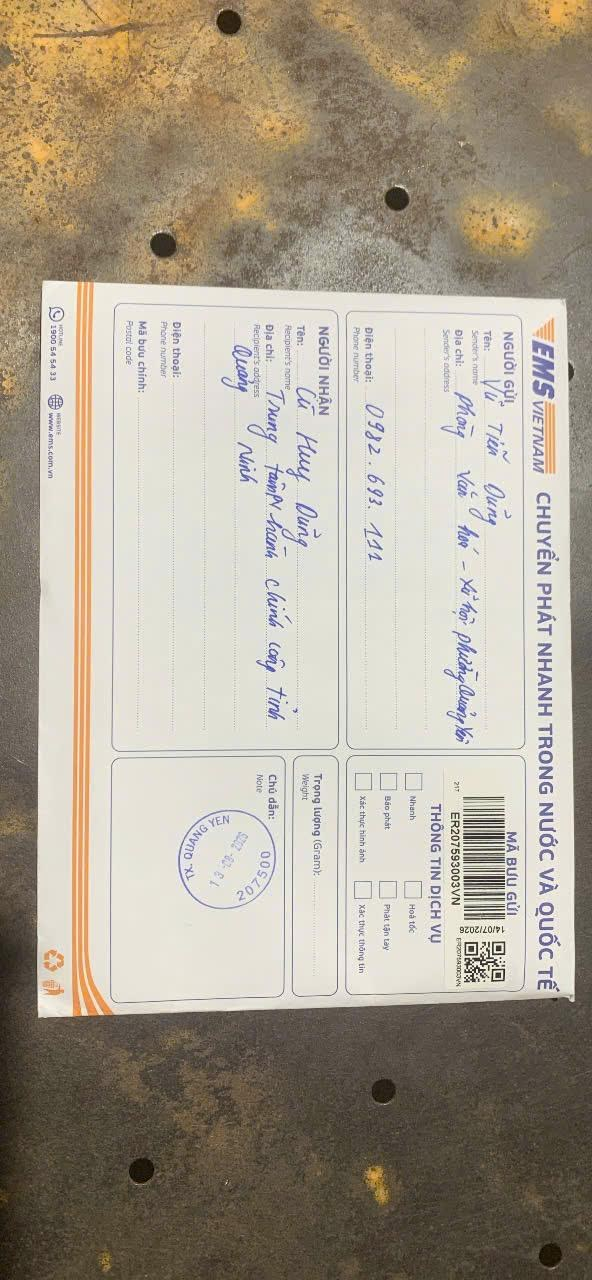
\includegraphics[height=6.2cm]{Images/fig3_1a.jpg}\hspace{0.6cm}
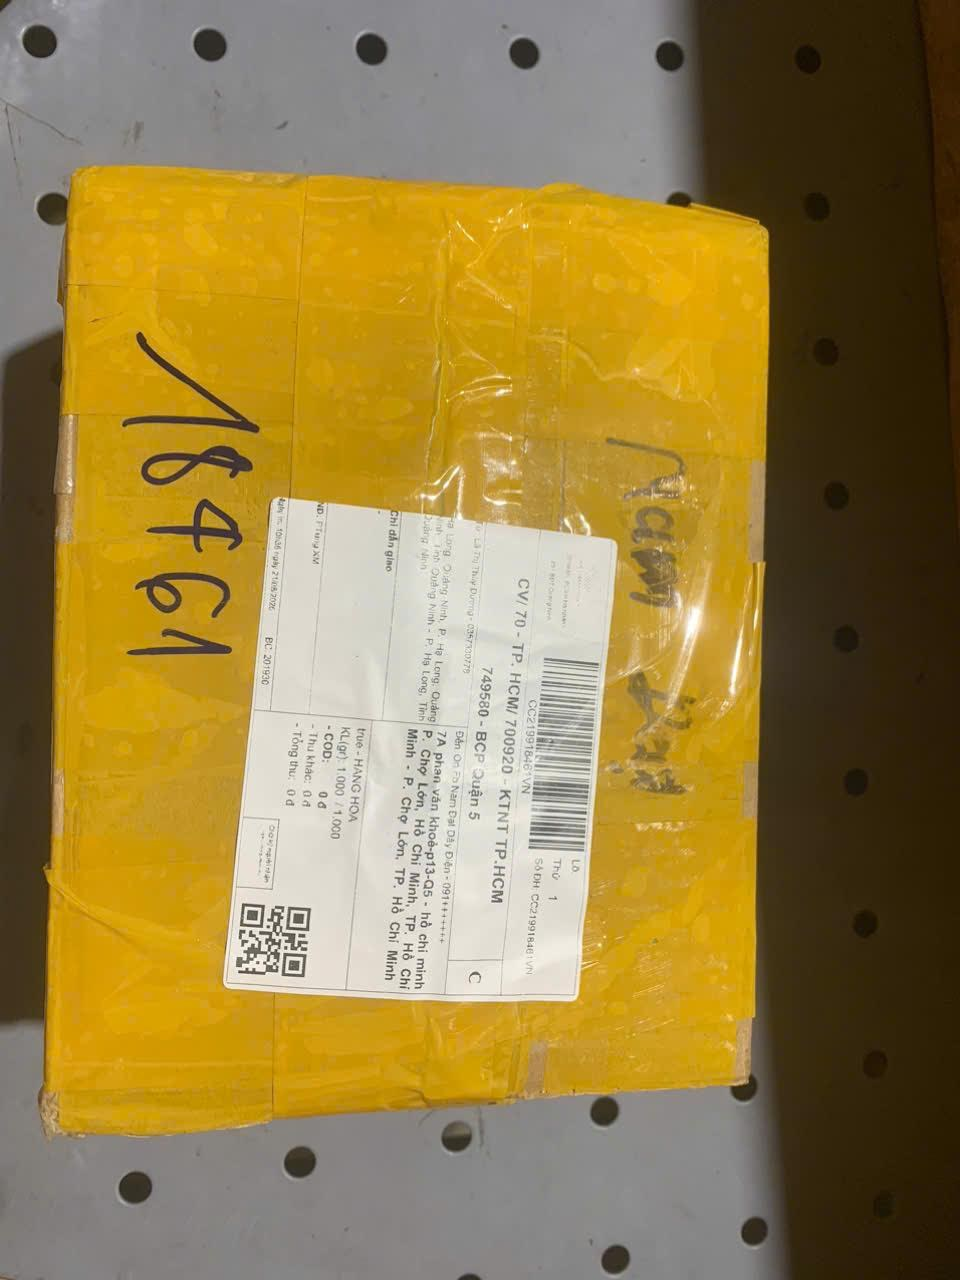
\includegraphics[height=6.2cm]{Images/fig3_1b.jpg}
\caption{Examples of annotated images in the Postal Item Dataset.}
\label{fig:postalitem}
\end{figure}

\begin{figure}[htbp]
\centering
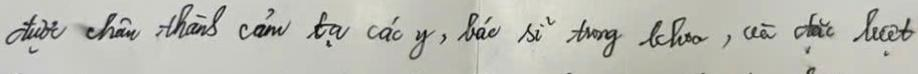
\includegraphics[width=0.9\textwidth]{Images/fig3_2a.jpg}\\[0.4cm]
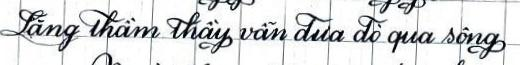
\includegraphics[width=0.9\textwidth]{Images/fig3_2b.png}
\caption[Examples of samples in Viet-Handwriting-OCR-v2]{Examples of samples in Viet-Handwriting-OCR-v2 \cite{viethandwriting}.}
\label{fig:viethandwriting}
\end{figure}

\begin{figure}[htbp]
\centering
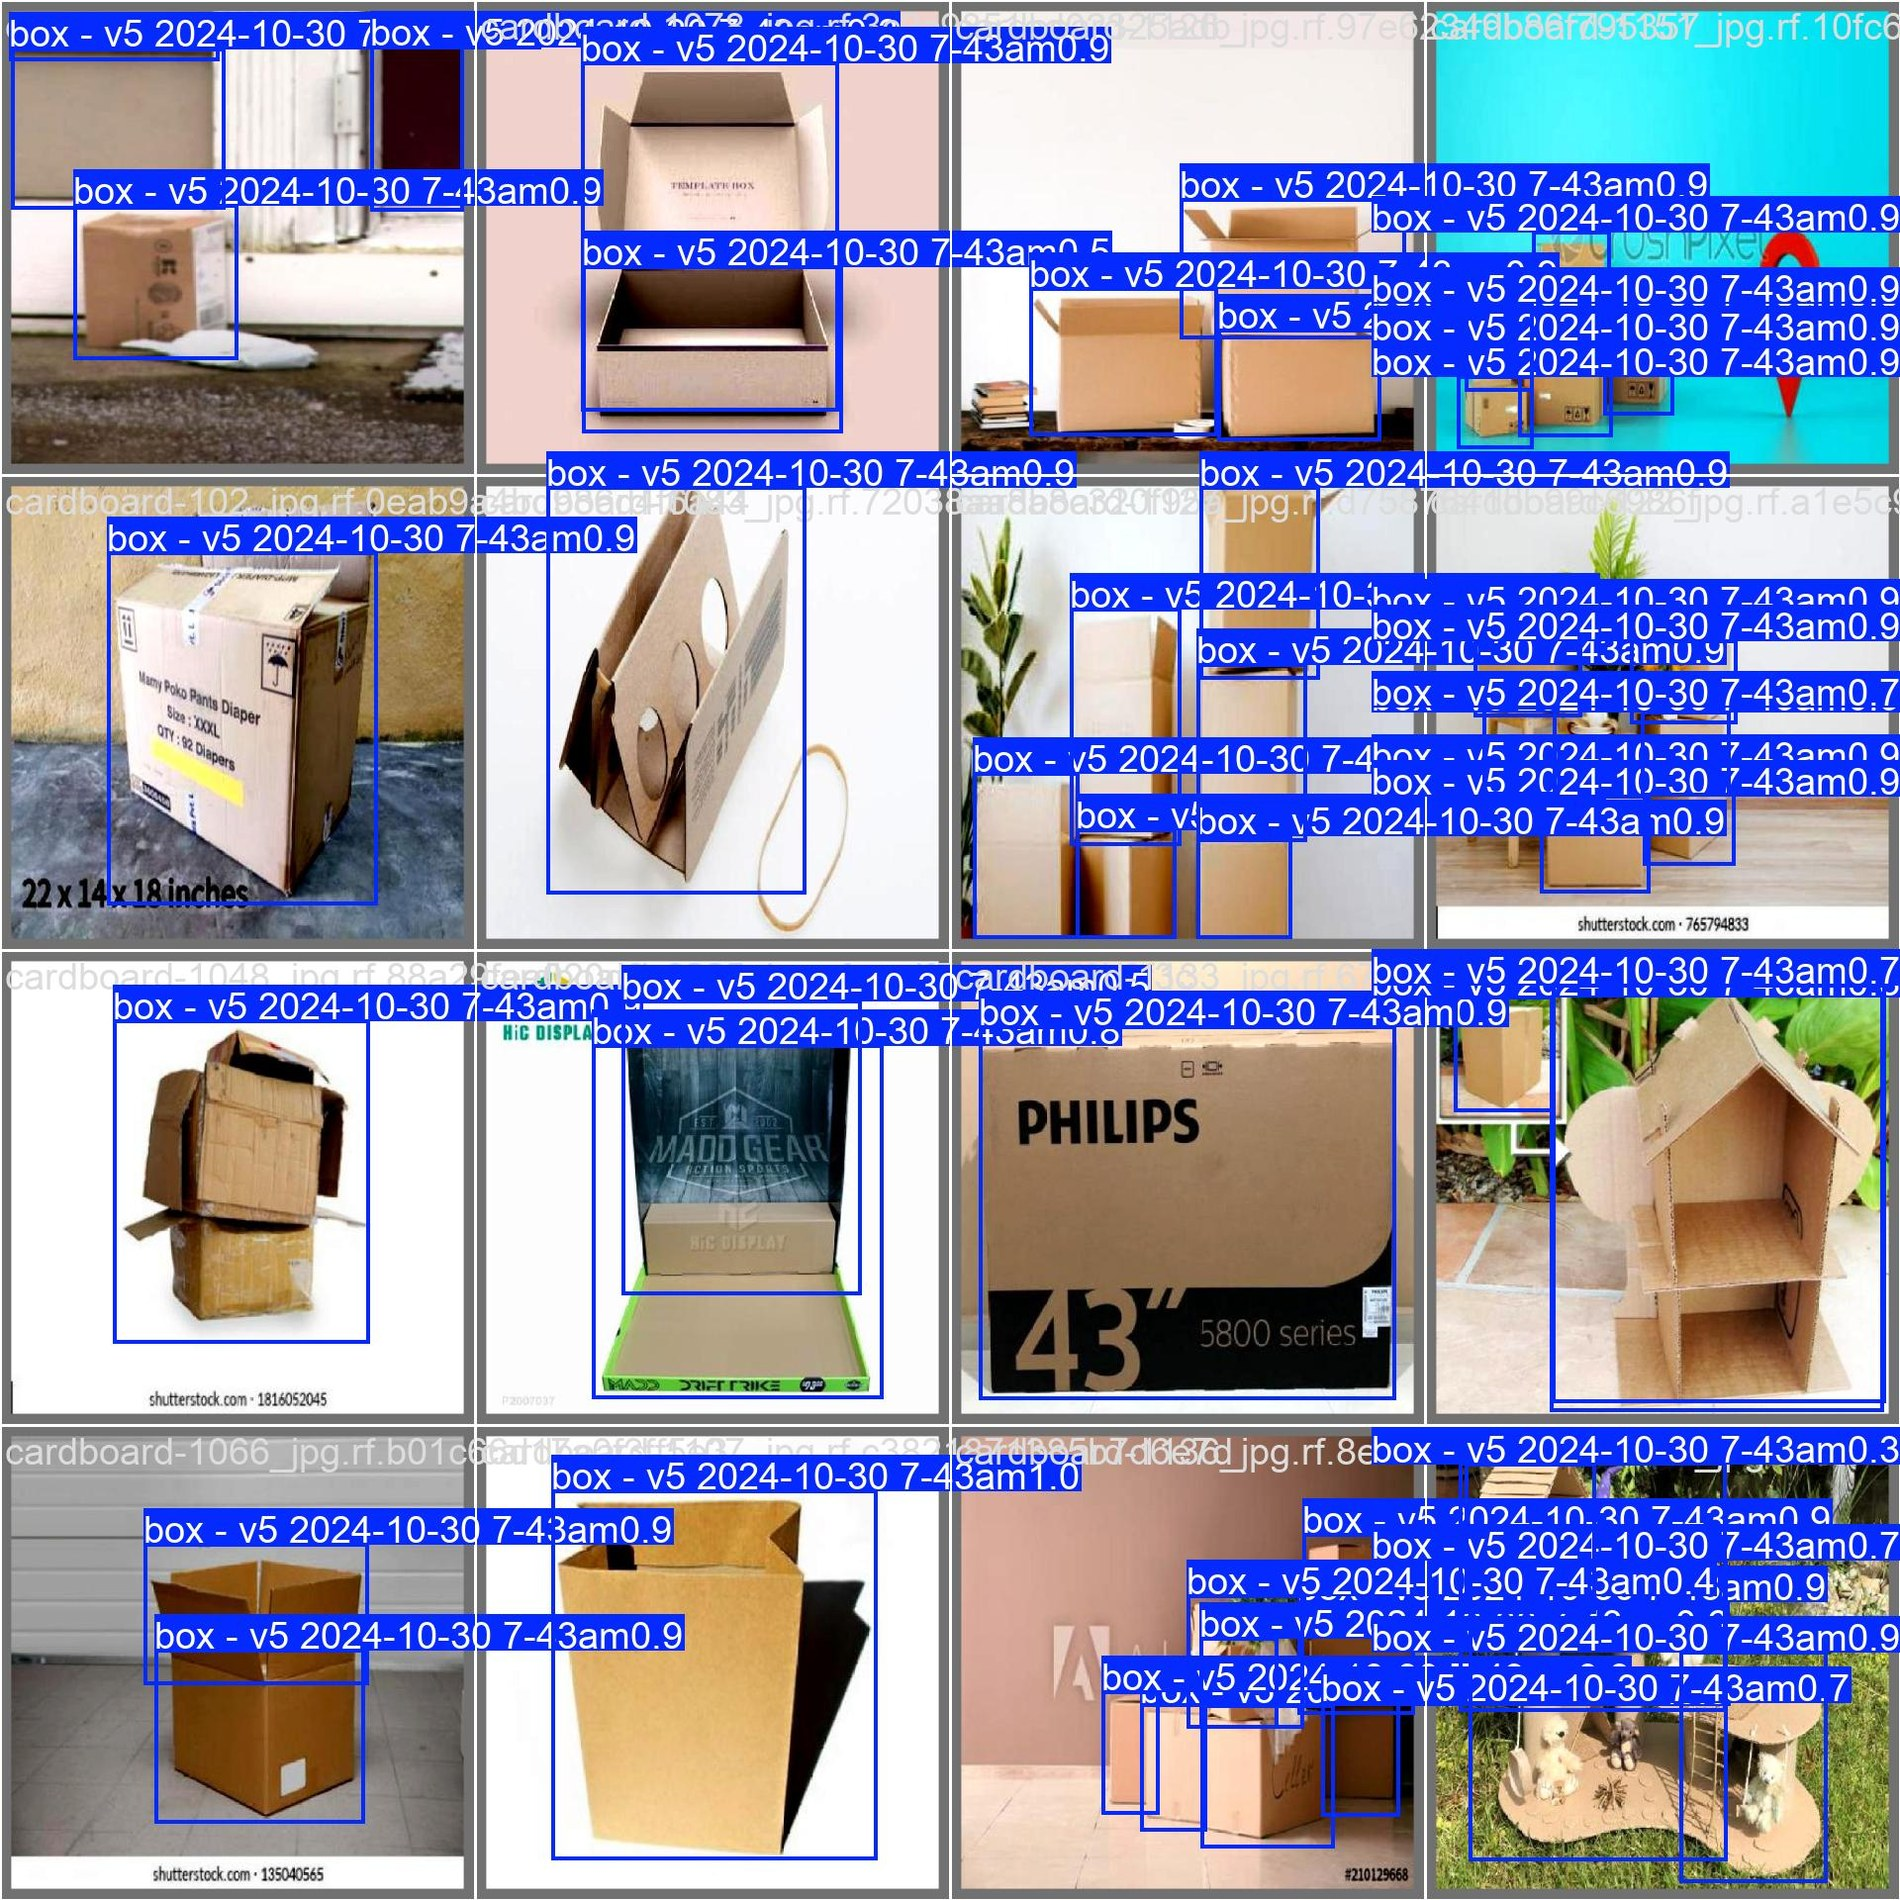
\includegraphics[width=0.72\textwidth]{Images/fig3_3.jpg}
\caption[Examples of annotated samples in the Cardboard Box Detection Dataset]{Examples of annotated samples in the Cardboard Box Detection Dataset \cite{cardboardbox2026}.}
\label{fig:cardboardbox}
\end{figure}

\begin{figure}[htbp]
\centering
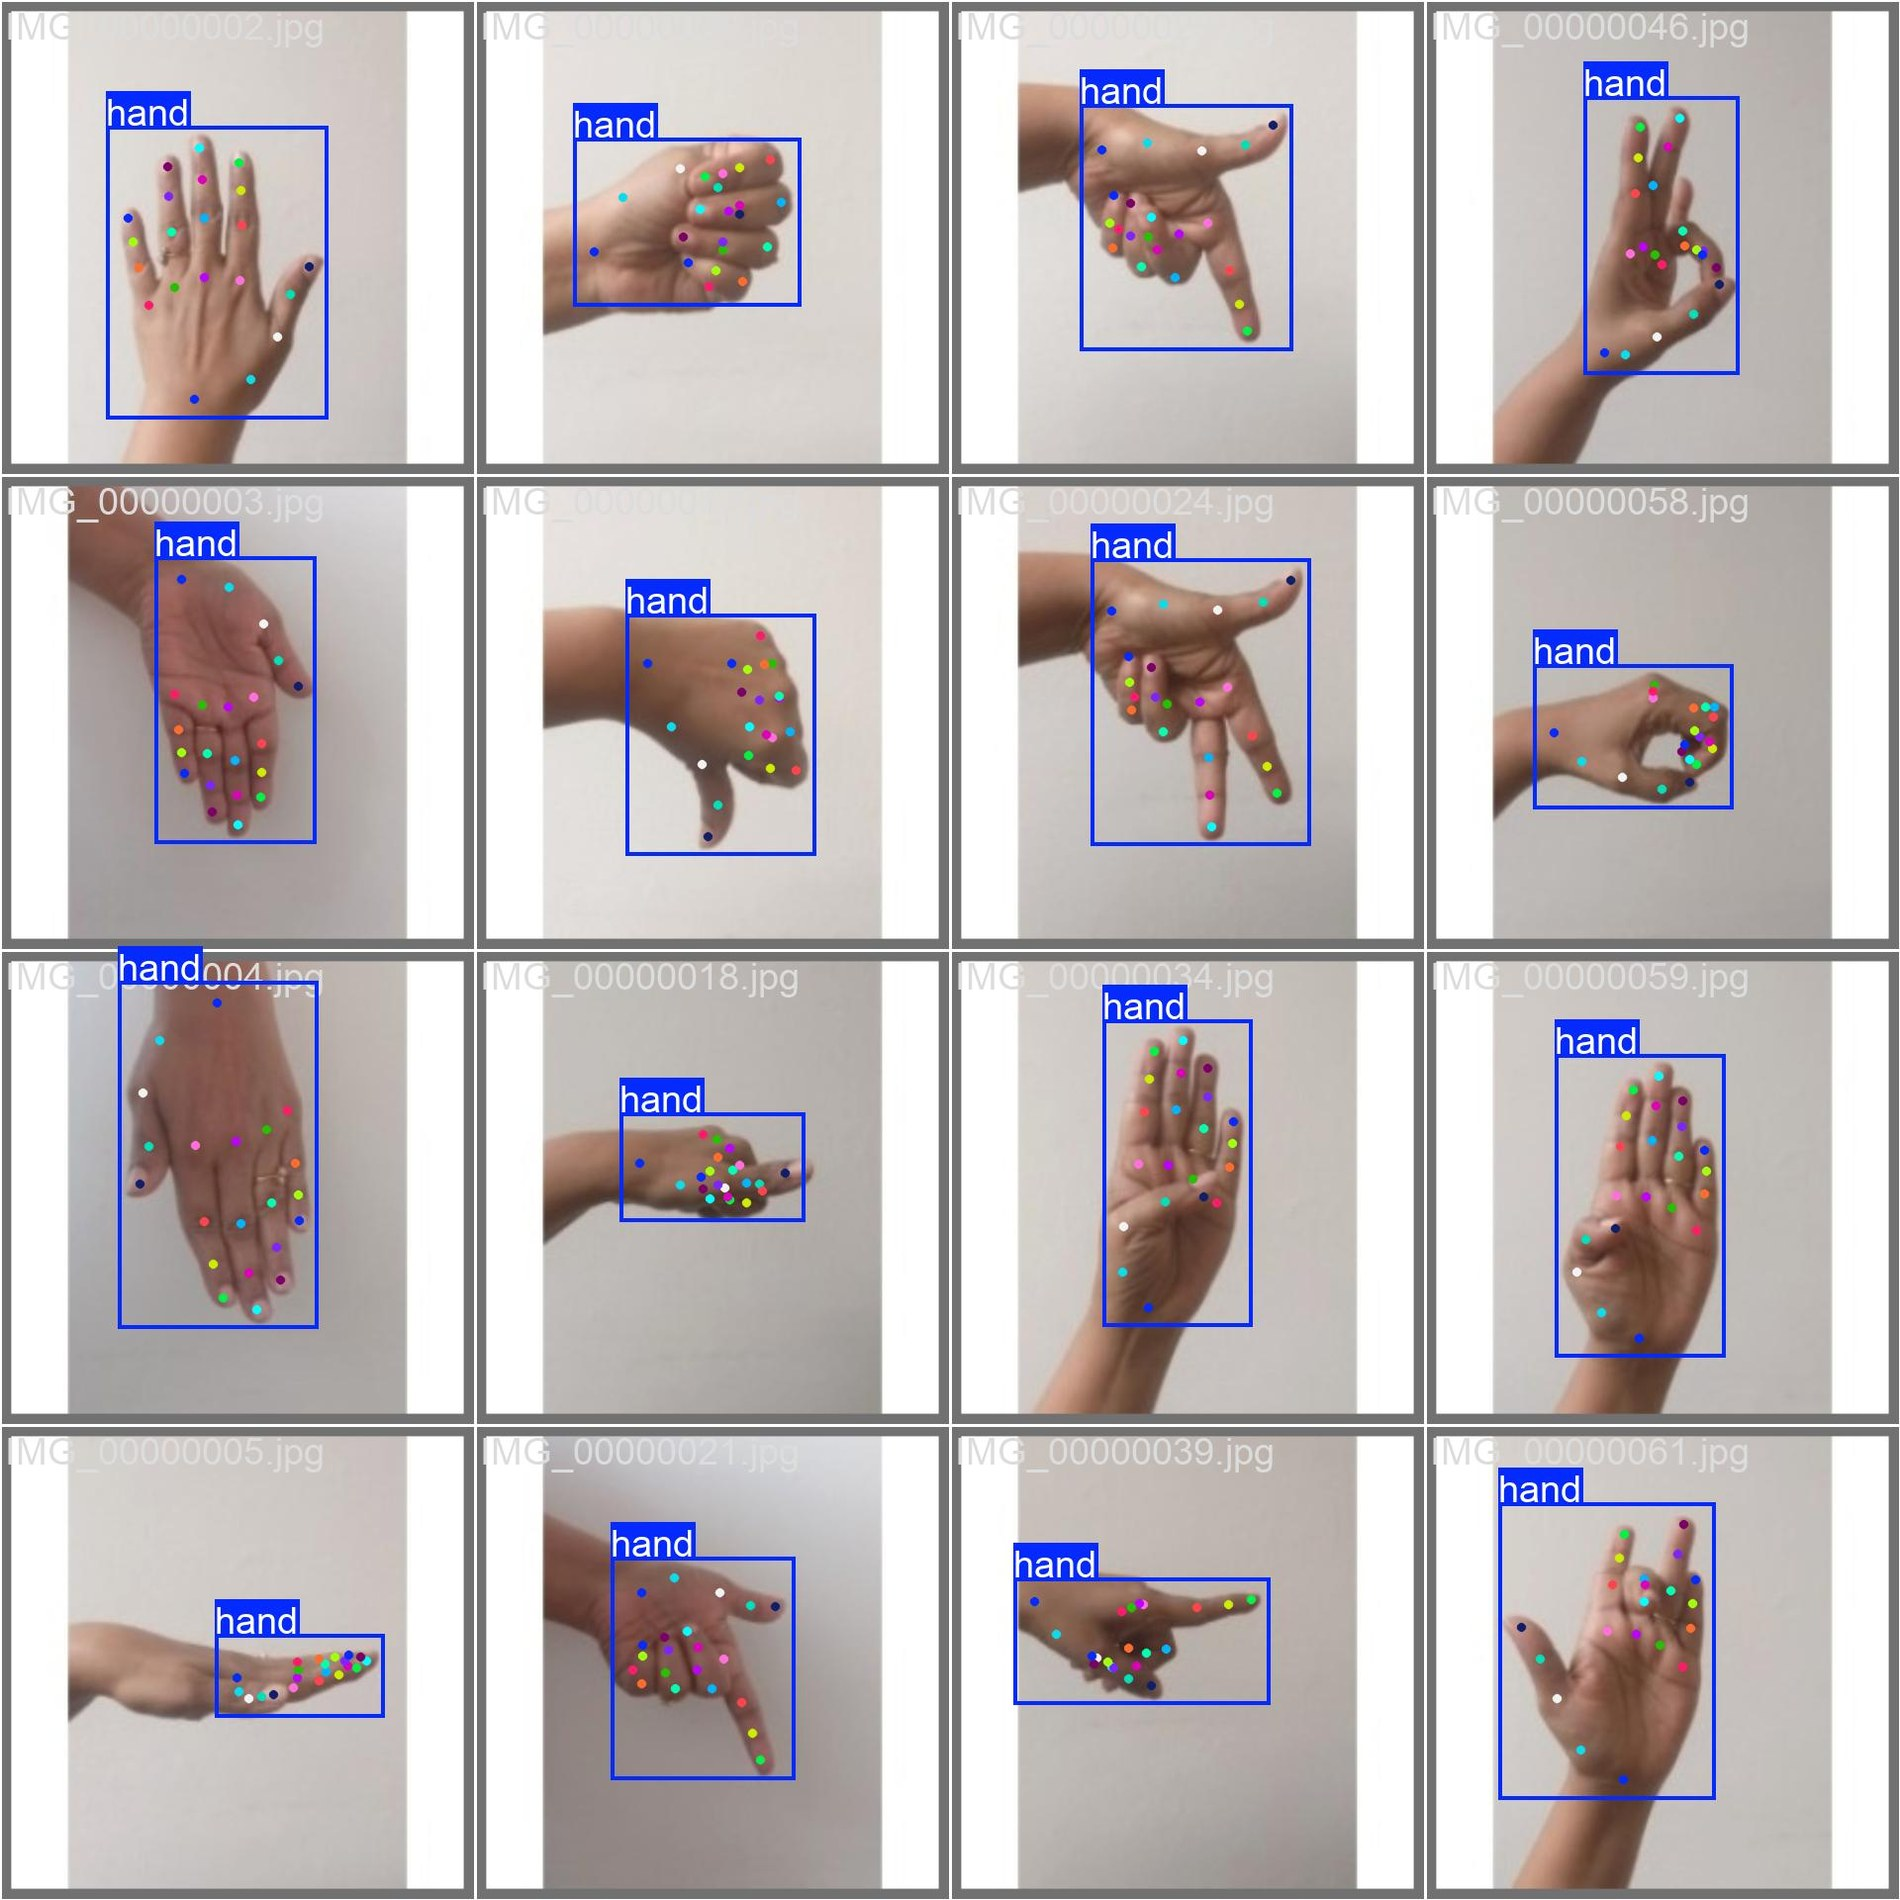
\includegraphics[width=0.72\textwidth]{Images/fig3_4.jpg}
\caption[Examples of annotated samples in the Hand Keypoints Dataset]{Examples of annotated samples in the Hand Keypoints Dataset \cite{ultralytics_hand}.}
\label{fig:handkeypoints}
\end{figure}

\section{Data Preprocessing and Cleaning}

Preprocessing was applied to the Postal Item Dataset only. The images in the training set were augmented to expand it from 351 to 1,050 images. The transformations include vertical flipping, rotation within $\pm 15^\circ$ and brightness adjustment within $\pm 15\%$. This process aims to increase the diversity of the training data. After augmentation, all images were resized to $640 \times 640$ pixels to provide a uniform input for the YOLO models.

For Box/Envelope Detection, the annotations were filtered to keep only the two classes \texttt{Label\_Box} and \texttt{Label\_Envelope}. For Information Region Detection, only images containing a \texttt{Label\_Box} were selected. The parcel region was cropped from the original image using the bounding box of the \texttt{Label\_Box} class, as illustrated in Figure~\ref{fig:cropinfo}. Cropping removes most of the background area and restricts the input data to the parcel surface.

\begin{figure}[htbp]
\centering
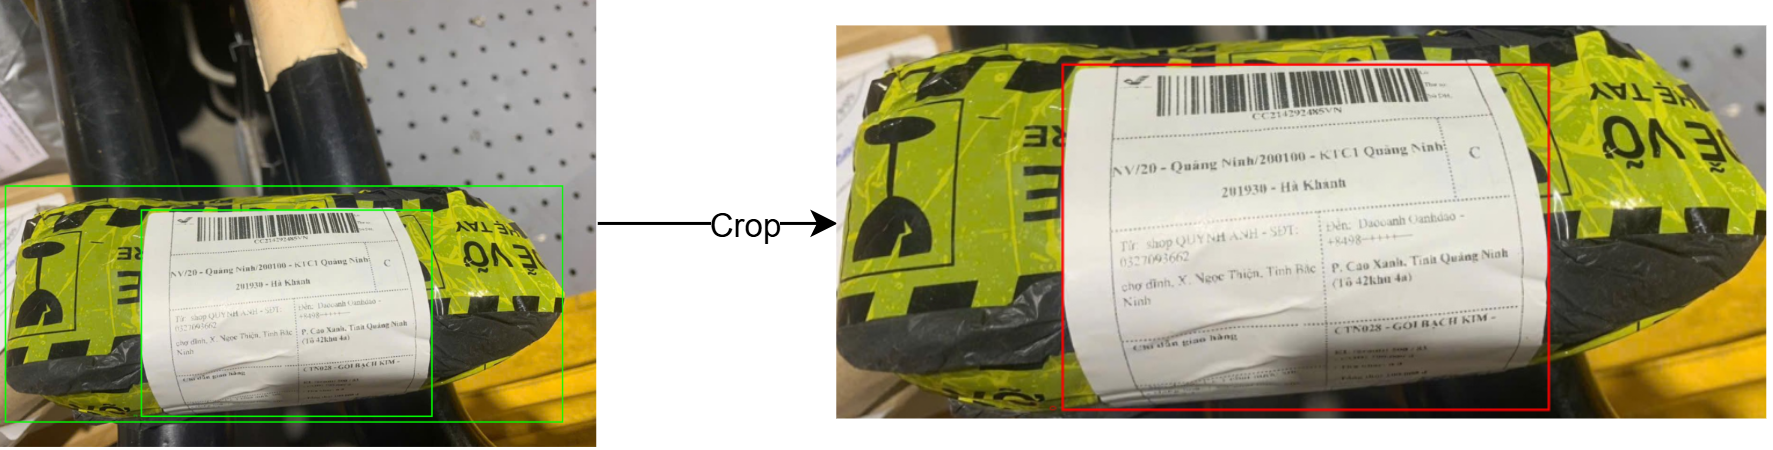
\includegraphics[width=\textwidth]{Images/fig3_5.png}
\caption{Illustration of the parcel region cropping process used to build the data for Information Region Detection.}
\label{fig:cropinfo}
\end{figure}

After the Label-Box region is cropped, the Label-info annotation in the original image can no longer be used directly, because the coordinate system of the image has changed. The bounding box coordinates of Label-info are therefore converted from the coordinate system of the original image to that of the cropped box image. From the bounding box $(x_c, y_c, W, H)$, the pixel coordinates are computed with Equation~\eqref{eq:pixelcoord}:

\begin{equation}
\label{eq:pixelcoord}
x = \left(x_c \pm \frac{W}{2}\right) W, \qquad
y = \left(y_c \pm \frac{H}{2}\right) H
\end{equation}

where $x_c$ and $y_c$ are the centre coordinates and $W$ and $H$ are the width and height of the image. From these, the edge coordinates of Label-info $[x_1{:}x_2,\, y_1{:}y_2]$ and of Label-box $[b_{x1}{:}b_{x2},\, b_{y1}{:}b_{y2}]$ are derived. After the box is cropped, the info coordinates are shifted into the new coordinate system with Equation~\eqref{eq:coordshift}:

\begin{equation}
\label{eq:coordshift}
x' = x - b_x, \qquad y' = y - b_y
\end{equation}

Once the four edge coordinates of the new Label-info are obtained, they are normalized back into YOLO format, and the class identifier is changed from 2, denoting \texttt{Label\_info}, to 0.

The remaining three datasets are fed into the models without any additional preprocessing beyond the default procedures of their sources.

\section{Summary of Data Processing}

The four datasets cover the main tasks of the system: distinguishing parcels from envelopes, detecting the information region, recognizing handwriting, detecting parcels and identifying hand regions. Preprocessing was limited to augmentation, resizing, annotation filtering, cropping and coordinate conversion on the self-collected Postal Item Dataset; the three public datasets were used as provided. The splits applied to each model are reported in Section~\ref{sec:training} together with the training configuration.

The Postal Item Dataset allows the models to learn the basic features needed to distinguish envelopes, parcels and information regions. However, the number of images is still limited. Cases such as deformed parcels or parcels with elongated shapes do not appear often enough, and the envelope images were mostly captured in the same environment and in a flat position, which reduces the diversity of the data.

Viet-Handwriting-OCR-v2 contains a relatively large number of samples and is suitable for fine-tuning the TrOCR model. However, the data was not built specifically for postal shipping forms, and the team did not apply augmentation to simulate real photographs. The model may therefore struggle with slanted handwriting, smudged ink or low-quality images.

Overall, the datasets provide a basis for training and evaluating each component of the system. Nevertheless, the quantity and diversity of real data from the post office still need to be expanded in order to cover deployment conditions more thoroughly.
